\documentclass[tikz,border=8pt]{standalone}
\usetikzlibrary{arrows.meta,positioning}
\begin{document}
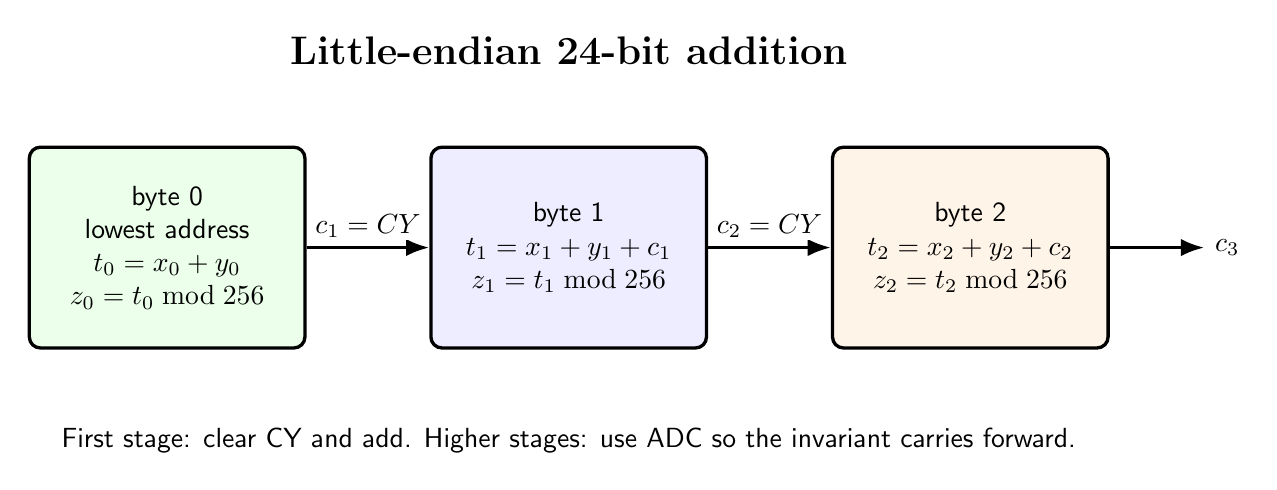
\begin{tikzpicture}[font=\sffamily,>=Latex,
 stage/.style={draw,very thick,rounded corners,minimum width=3.5cm,minimum height=2.55cm,align=center,inner sep=7pt}]
\node[font=\Large\bfseries] at (7.0,5.3) {Little-endian 24-bit addition};
\node[stage,fill=green!8] (s0) at (1.9,2.8) {byte 0\\lowest address\\$t_0=x_0+y_0$\\$z_0=t_0\bmod256$};
\node[stage,fill=blue!7] (s1) at (7.0,2.8) {byte 1\\$t_1=x_1+y_1+c_1$\\$z_1=t_1\bmod256$};
\node[stage,fill=orange!9] (s2) at (12.1,2.8) {byte 2\\$t_2=x_2+y_2+c_2$\\$z_2=t_2\bmod256$};
\draw[very thick,->] (s0)-- node[above=2pt,fill=white,inner sep=1pt] {$c_1=CY$} (s1);
\draw[very thick,->] (s1)-- node[above=2pt,fill=white,inner sep=1pt] {$c_2=CY$} (s2);
\draw[very thick,->] (s2.east)--++(1.2,0) node[right] {$c_3$};
\node[align=center] at (7.0,.35) {First stage: clear CY and add. Higher stages: use ADC so the invariant carries forward.};
\end{tikzpicture}
\end{document}
